\documentclass[10pt]{article}
% Puedes usar esto (u otra codificaci\'on) si quieres:
\usepackage{graphicx}
\usepackage[utf8]{inputenc} %para usar acentos por ejemplo
\usepackage[spanish]{babel}  % para que las directivas del latex se impriman en españos. Por ejemplo \begin{abstract} ... \end{abstract}, aparecería "Abstract", pero con este paquete aparecerá "Resumen"
\usepackage{imakeidx}
\usepackage{listings}
\usepackage{float}
\usepackage{hyperref}

\makeindex[columns=3]

\title{Metaheurísticas Poblacionales} % El titulo debería ser lo mas descriptivo y conciso posible
\author{Rosas Francisco, Gurruchaga Luciano}

\date{\today} % Eliminar \today y no pone la fecha actual según se indica: \date{}

\begin{document}

% Agrega el título
\maketitle

\begin{abstract}

El objetivo de este documento será el estudio, analisis y comparación de dos algoritmos metaheuristicos poblacionales, Algoritmo Genético \textbf{GA} y Evolución Diferencial  \textbf{DE}. Los mismos serán sometidos a una serie de pruebas en funciones complejas conocidas  \textit{Ackley 1, Ackley 2, Ackley 3 y Ackley 4 }con variacion en el tamaño de las dimensiones. Luego, se verá el desepeño de dichos algoritmos descubriendo cual es el metodo mas adecuado para la resolucion de problemas en un espacio grande de soluciones complejas de optimizar. 
Debido a esta problematica, se comenzará con la definicion de conceptos básicos necesarios, alguna mención del estado del arte al día de la fecha, y expondremos las  implementaciones y consideraciones de las soluciones. Finalmente se procedera a la comparacion de los resolutados del objeto de estudio y por que  \textbf{DE} es novedoso.

\end{abstract}

%----------------------------------------------------------------------------------------
%	Contenido del artículo
%----------------------------------------------------------------------------------------

\section{Introducción}
\subsection{\textbf{GA}- Algoritmo Genético }

Los Algoritmos Geneticos conocidos como GA por sus siglas en ingles Genetic Algorithm, son una analogía a la selección natural, es decir, que estan inspirados en ella.

\t Se trabaja con un conjunto de soluciones al que llamaremos \textbf{poblacion}, cada solucion particular o \textbf{individuo} es representada por medio de un vector de valores discretos llamado \textbf{cromosomas}. A los simbolos que conforman dichos vectores se les llama \textbf{genes}. Los cromosomas evolucionan a lo largo de distintas iteraciones, las llamadas \textbf{generaciones}. En cada generacion, los cromosomas son evaluados usando alguna medida de aptitud o funcion objetivo. Las siguientes generaciones, nuevos cromosomas, son generadas aplicando operadores genéticos repetidamente a la generacion actual, siendo estos los operadores de selección (selection), cruzamiento (crossover), mutación (mutation) y reemplazo.

\subsection{\textbf{DE}- Evolución Diferencial }
\t En la computación evolutiva (  Familia de algoritmos de optimización global inspirados en la evolución biológica - rama de la Inteligencia Artificial )[2], evolución diferencial es un método que optimiza un problema intentando mejorar una solucion candidata iterativamente con respecto a una medida de calidad determinada. Estos metodos son comunmente conocidos como "Metaheuristicas", ya que no hace ninguna suposición(o muy pocas)  sobre el problema que se está optimizando y puede buscar espacios muy grandes de soluciones candidatas. Sin embargo, las metaheuristicas como DE no garantizan encontrar la solucion optima.

\t  DE es usado para funciones multidimencionales de valores Reales, sin utilizar el "gradiente" del problema a ser optimizado, en otras palabras, \textbf{DE} no requiere o no necesita que el problema a optimizar sea diferenciable, como en el clasico caso del metodo de "descenso del gradiente" [3] o "Quasi-Newton method" [4]. Por lo tanto, la evolucion diferencial también puede utilizarse en problemas de optimización que ni siquiera son continuos, son ruidosos, cambian con el tiempo, etc.
\t La ED optimiza un problema manteniendo una población de soluciones candidatas y creando nuevas soluciones candidatas combinando las existentes según sus sencillas fórmulas, y quedándose con la solución candidata que tenga la mejor puntuación o aptitud en el problema de optimización en cuestión. De este modo, el problema de optimización se trata como una caja negra que simplemente proporciona una medida de calidad dada una solución candidata y, por tanto, el gradiente no es necesario.

\t La ED fue introducida por Storn y Price en la década de 1990. Se han publicado libros sobre los aspectos teóricos y prácticos del uso de la ED en la computación paralela, la optimización multiobjetivo y la optimización restringida, ymuchos otros estudios en diversas áreas de aplicación. 

\subsection{Funciones Akcley}

Las funciones de prueba son importantes para validar y comparar el rendimiento de los algoritmos de optimización algoritmos de optimización. En la literatura se han publicado muchas funciones de prueba o de referencia; Sin embargo, no existe una lista o conjunto estándar de funciones de referencia. Lo ideal es que las funciones de prueba deben tener diversas propiedades para que puedan ser realmente útiles para probar nuevos algoritmos de una
de forma imparcial.

La comprobación de la fiabilidad, la eficiencia y la validación de los algoritmos de optimización se lleva a cabo con frecuencia utilizando un conjunto elegido de puntos de referencia estándar comunes o funciones de prueba de la literatura. El número de funciones de prueba en la mayoría de los artículos varía entre unas pocas y unas dos docenas. Lo ideal sería que las funciones de prueba utilizadas fueran diversas e insesgadas, pero no existe un conjunto de funciones de prueba acordado en la literatura. Por lo tanto, el principal objetivo de este artículo es revisar y recopilar el conjunto más completo de funciones de prueba que podemos encontrar en toda la de todas las publicaciones disponibles, de modo que puedan utilizarse para la futura validación y comparación de los algoritmos de optimización. algoritmos de optimización.

En general, los problemas sin restricciones pueden clasificarse en dos categorías: funciones de prueba y los problemas del mundo real. Las funciones de prueba son problemas artificiales, y pueden utilizarse para evaluar el comportamiento de un algoritmo en situaciones a veces diversas y difíciles. Los problemas artificiales pueden incluir un único mínimo global, uno o varios mínimos globales en presencia de muchos mínimos locales, valles largos y estrechos, efectos de espacio nulo y superficies planas. Estos problemas pueden ser fácilmente manipulados y modificados para probar los algoritmos en diversos escenarios. Por otro lado, los Por otra parte, los problemas del mundo real se originan en diferentes campos como la física, la química ingeniería, matemáticas, etc. Estos problemas son difíciles de manipular y pueden contener expresiones algebraicas o diferenciales complicadas y pueden requerir una cantidad significativa de de datos para compilarlos.

En el presente trabajo, nos centraremos en los puntos de referencia de la función de prueba y sus diversas propiedades como la modalidad y la separabilidad. Una función con más de un óptimo local se denomina multimodal. Estas funciones se utilizan para probar la capacidad de un algoritmo para escapar de cualquier mínimo local. Si el proceso de exploración de un algoritmo está mal diseñado
entonces no puede buscar el paisaje de funciones de manera efectiva. Esto, a su vez, hace que un algoritmo se quede atascado en un mínimo local. Las funciones multimodales con muchos mínimos locales se encuentran entre la clase de problemas más difícil para muchos algoritmos. Las funciones con superficies planas suponen una
dificultad para los algoritmos, ya que la planitud de la función no da al algoritmo ninguna información para dirigir el proceso de búsqueda hacia los mínimos (Stepint, Matyas, PowerSum).
Otro grupo de problemas de prueba está formulado por funciones separables y no separables. Según [16], la dimensionalidad del espacio de búsqueda es una cuestión importante del problema. En algunas funciones, el área que contiene ese mínimo global es muy pequeña, cuando se compara con todo el espacio de búsqueda, como Easom, Michalewicz (m=10) y Powell. En problemas como Perm, Kowalik y Schaffer, el mínimo global se encuentra muy cerca de los mínimos locales. Si el algoritmo no puede mantener los cambios de dirección en las funciones con un valle curvo estrecho, en el caso de funciones como Beale, Colville, o no puede explorar el espacio de búsqueda de forma efectiva, en el caso de funciones como Pen Holder, Testtube-Holder que tienen múltiples mínimos globales, el algoritmo fallará para este tipo de problemas. Otro problema que algoritmos pueden sufrir es el problema de la escala con muchos órdenes de magnitud diferencias entre el dominio y la hiper-superficie de la función [47], como Goldstein-Price y Trid.

Las funciones ackley son funciones muy fieras por que le hacen nana a los GA.[5]


\section{Descripción del Problema}
En el problema  de Strip Packing (SPP) o empaquetado de tiras bidimensionales tenemos, una tira de anchura finita W pero de altura infinita, y un conjunto de elementos rectangulares de anchura máxima W. 
	El objetivo es empaquetar todos los elementos en la tira para minimizar la altura utilizada. Los elementos no pueden solaparse ni girarse(estudiaremos un caso en el que si puedan rotar). 
Dentro del mismo nivel, todos los elementos se empaquetan de forma que sus fondos queden alineados. El primer nivel es el fondo de la tira y los niveles siguientes se definen por la altura del artículo más alto del nivel anterior.
	Este es un problema de mucho interes de estudio ya que forma parte del a familia de problemas $NP-Hard$, es decir no se ha encontrado una solución en un tiempo polinomico.

\subsection{Definicion:}
%$  X  $
Una instancia $ I = (R,W)$  del problema de empaquetado de tiras consiste en una tira con anchura $W = 1$ y altura infinita, así como un conjunto $R$  de elementos rectangulares. Cada elemento $r   \in   R$ tiene una anchura  $w_r \in  (0,1]  \cap  Q $ y una altura  $h_r     \in   (0,1] \cap Q $. Un empaquetamiento de los elementos es un mapeo en cada esquina inferior izquierda de un elemento $r    \in   R$  a una posición $(x_r,y_r) \in([0,1 - w_r] \cap Q) \times Q\geq 0$ en el interior de la franja. 
Un punto interior de un elemento colocado $ r \in  R $ es un punto del conjunto $inn(r)={(x,y) \in Q\times Q | x_r < x_r + w_r , y_r<y_r+h_r}$ .
Dos elementos (colocados) se solapan si comparten un punto interior. La altura del empaquetamiento se define como $ \max \{ y_r + h_r | r \in R\} $. El objetivo es encontrar un empaquetamiento libre de solapamiento de los elementos dentro de la franja minimizando la altura del empaquetamiento.

 En este informe utilizaremos una serie de instancias 
contenidas en ("spp9a.txt", "spp9b.txt", "spp10.txt", "spp11.txt", "spp12.txt", "spp13.txt") las cuales varian en su conjunto $R$ y en $W$.

\section{Propuesta algorítmica} % El titulo de esta y el resto de las secciones es orientativa

\t Una forma comun de atacar este problema es el enfoque orientado al nivel, los rectangulos se insertan de izquierda a derecha, en filas que forman niveles. Dentro del mismo nivel, todos los elementos se empaquetan de forma que sus fondos se alineen. El primer nivel es el fondo de la tira y los niveles siguientes se definen por la altura del rectangulo más alto del nivel anterior.
 
\t Algunos algoritmos comienzan ordenando los artículos por altura no creciente, suelen denominarse de altura decreciente \textbf{DH}, y orientados al nivel. Varaciones de dicho algoritmo son los algoritmos First-Fit Decreasing Height \textbf{FFD}, Next-Fit Decreasing Height \textbf{NFD} y Best-Fit Decreasing Height \textbf{BFDH}.[5]

Existen muchas mas variaciones, nosotros utilizaremos un enfoque orientado al nivel, pero en vez de ordenar los elementos por su altura, utilizaremos un enfoque metaheuristico poblacionall, mas precisamente un algoritmo genetico que encuentre una solucion aproximada aceptable a nuestro problema.

\subsection{¿Que es un Algoritmo Genetico?}

Un algoritmo genetico es una metaheuristica poblacional inspirada en el proceso de la seleccion natural.

Contamos con una poblacion $P$, dicha poblacion esta formada por un conjunto de soluciones individuos $I$, cada individuo $I$ esta representado por un conjunto de cromosomas, los cuales a su vez estan formados una secuencia de genes $g_i$ de valor discreto, que representan una solucion al problema, formalmente:

$$P =\{i_0,i_1,..,i_n\}$$
$$I =\{(g_0,g_1,..,g_n)_0,(g_0,g_1,..,g_n)_1,...,(g_0,g_1,..,g_n)_n\}$$

Se toman todos los individuos de la poblacion $I \in P$, se obtiene una medida de "desempeño" de cada solucion $I$, aquellos con mejor desempeño son mas propensos a reproducirse, como sucede en la seleccion natural donde los mas aptos sobreviven y tienen mas posibilidades de trasmitir sus genes.

Existen distintas formas de seleccionar que individuos se reproducen, nosotros utilizaremos la \textit{"seleccion basada en torneos"} la cual consiste en seleccionar de forma aleatoria dos individuos distintos de la poblacion, y , aquel con mejor desempeño sera quien pueda reproducirse y por tanto sus genes seran "heredados" en la siguiente poblacion $P$. Sumado a esto existe una probabilidad de cruza y mutacion de los genes al reproducirse.

Para la primera utilizaremos el operador de cruce \textbf{PMX} o \textit{cruce por emparejamiento parcial}. Consiste en elegir un subsegmento de los genes de uno de los progenitores y cruzarlos preservando el orden y la posición de la mayor cantidad de genes posible del otro manteniendo la coherencia.
En cuanto a la mutacion utilizaremos una \textit{permutacion simple} entre dos genes aleatorios $g_i,g_j$ del mismo individuo.

A medida que avanzan las generaciones, en cada poblacion iran quedando aquellos individuos que cuentan con los "mejores"  genes de generaciones anteriores, por tanto los de mejor desempeño. Recuperando al mejor individuo historico (de todas las generaciones) obtenemos una solucion aproximada aceptable.

\subsection{Aplicacion a SPP}
En nuestro caso particular contaremos con diferentes $(R,W)$ por achivo. Los cuales representan un $W$ y serie de rectangulos $r_i \in R$ donde $R$ es el conjunto de rectangulos totales que conforman nuestro problema. Si tomamos una secuencia ordenada de rectangulos particular $S_i = (r_0,r_1,..,r_n)$, la cual representa el orden de insercion de los rectangulos a la hora de realizar el corte, obtendremos asi una solucion o individuo si tomamos dicha secuencia $S_i$ como un cromosma de $I_i$, la posicion de cada rectangulo en el cromosoma es un gen:

$$I_i = S_i$$
$$S_i = (r_0,r_1,..,r_n)$$
$$I_i = \{(r_0,r_1,..,r_n)\}$$

En nuestro problema particular veremos la diferencia entre aplicar un enfoque sin rotacion y con rotacion, para la representacion del estado de cada rectangulo en la solucion (girado o no girado) utilizaremos nuevo cromosoma con la forma de un vector mascara $Mr$ el cual estara formado por una secuencia de valores booleanos $(b_0, b_1,...,b_n)$ donde $b_i$ indica si $r_i \in I$ esta rotado o no, luego la solucion $$I_i$$ es un par ordenado de la forma:

$$I_i = \{S_i,Mr_i\}$$
$$S_i = (r_0,r_1,..,r_n)$$
$$Mr_i = (m_0, m_1,...,m_n)$$

%PRIMERO ANCHO, DESPUES ALTURA

Por ejemplo, si tuvieramos un conjunto de rectangulos $r_0=(2,2),r_1=(5,2),r_2=(3,5), r_3 = (3,1), r_4=(2,4)\in R$, un ancho de tira $W = 7$, la solucion $I_0 = \{S_0,Mr_0\}$ con la forma $S_0 = (r_0,r_1,r_2,r_4,r_3), Mr_0 = (0,0,1,0,1)$ es:

%\begin{figure}[H]
%\centerline{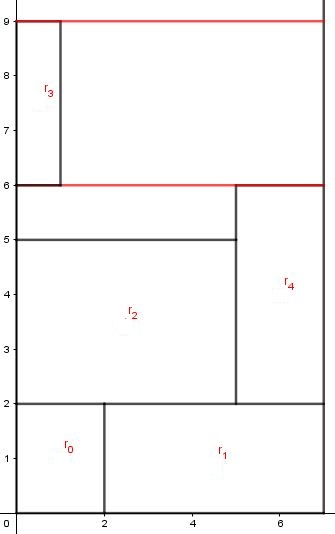
\includegraphics[width=0.7\linewidth]{grafica_ejemplo_solucion_GA.jpg}}
%\caption{Representacion grafica de la solucion $I_0$}
%\label{fig_1}
%\end{figure}

Evaluaremos el desempeño de las soluciones en base a la menor altura de dicha solucion, por ejemplo, si tomamos la solucion $I_0$, su desempeño seria $f(I_0) = 9$ en cambio una solucion $I_1 = \{S_1,Mr_1\}$ con la forma $S_1 = (r_1,r_2,r_0,r_3,r_4), Mr_1 = (0,0,0,0,0)$, tendria un desempeño $f(I_1) = 11$, con dicho criterio de evaluacion podemos decir que $I_0$ es mejor solucion al problema que $I_1$ y por tanto es mas probable de ser seleccionada para reproducirse y volverse progenitora de individuos en siguientes generaciones.

%\begin{figure}[H]
%\centerline{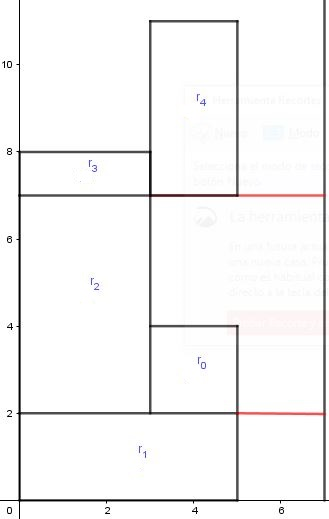
\includegraphics[width=0.7\linewidth]{grafica_ejemplo_solucion2_GA.jpg}}
%\caption{Representacion grafica de la solucion $I_1$}
%\label{fig_2}
%\end{figure}

Supongamos ahora que vamos a reproducir ambas soluciones $I_0,I_1$. Recordemos que existia una probabilidad asociada a la mutacion como al evolucionar. Si dichas probabilidades no se cumplen (los hijos no evolucionan ni mutan) simplemente heredaran los genes de sus progenitores, el hijo $H_0 = I_0, H_1 = I_1$, los progenitores "pasarian" a la siguiente generacion sin cambios.

En caso de que se produzca un cruce (evolucion) el operador PMX trabajara con ambos progenitores de la siguiente forma: 
Se toma un intervalo aleatorio en el cromosoma de la solucion, por ejemplo $b = [1,3]$ en $I_0$ el rango abarcaria $S_0[1,2] = (r_0,r_1), Mr_0[1,2] = (0,0)$ y en $I_1$, $S_1[1,3] = (r_1,r_2), Mr_1[1,2] = (0,0)$.

Generamos dos hijos $H_0 = I_0, H_1 = I_1$, tomamos los genes del intervalo
$$H_0[1,2] = \{(r_0,r_1),(0,0)\}, H_1[1,2] = \{(r_1,r_2),(0,0)\}$$

Intercambiamos los genes con el progenitor opuesto:
$$H_0[1,2] = I_1[1,2] = \{(r_1,r_2),(0,0)\}, H_1[1,2] = I_0[1,2] = \{(r_0,r_1),(0,0)\}$$ 

Los hijos nos quedan de la forma: 
$$H_0=\{(r_1,r_2,r_2,r_4,r_3),(0,0,1,0,1)\}, H_1 = \{(r_0,r_1,r_0,r_3,r_4),(0,0,0,0,0)\}$$

Podemos ver que los rectangulos $r_2, r_0$ se encuentran repetidos en $H_0$ y $H_1$ respectivamente, para corregir esto tomamos aquellos genes repetidos que quedaron fuera del intervalo $b$ en este caso el tercer gen de cada cromosoma y lo reemplazamos por un rectangulo aleatorio faltante $r_0, r_2$ respectivamente, obteniendo como resultado:
$$H_0=\{(r_1,r_2,r_0,r_4,r_3),(0,0,0,0,1)\}, H_1 = \{(r_0,r_1,r_2,r_3,r_4),(0,0,0,0,0)\}$$

Ahora dado que al recuperar el rectangulo faltante en cada hijo, lo insertamos por defecto, es decir, sin rotar, tomaremos el tercer gen del cromosoma $Mr_i$ y lo reemplazaremos por un valor booleano aleatorio, nos quedaria de la siguiente forma:
$$H_0=\{(r_1,r_2,r_0,r_4,r_3),(0,0,0,0,1)\}, H_1 = \{(r_0,r_1,r_2,r_3,r_4),(0,0,1,0,0)\}$$

Suponiendo una mutacion en alguno de los hijos, $H_0$, simplemente permutamos dos genes y su valor booleano respectivo, por ejemplo intercambiamos $r_1,r_3$ y $m_0,m_4$ en $H_0$ obteniendo:
$$H_0=\{(r_3,r_2,r_0,r_4,r_1),(1,0,0,0,0)\}$$

Tambien mutaremos el cromosoma $M_0$ independiente de $S_0$, por ejemplo $m_0,m_1$:
$$H_0=\{(r_3,r_2,r_0,r_4,r_1),(0,1,0,0,0)\}$$

Con estas bases podemos encarar el problema de forma general, recordando: 
Un problema, $R = \{r_0,r_1,..,r_n\}$
Una poblacion inicial $P_0={i_0,i_1,...,i_k}$ donde cada individuo es de la forma:
$I_i = \{S_i,Mr_i\}$ donde $S_i = (r_0,r_1,..,r_n), Mr_i = (m_0, m_1,...,m_n)$, $|R| = |S_i| = |Mr_i|$

A cada inviduo $I_j \in P_i$ se lo evaluara en funcion a su altura total (se considerara o no el valor booleano respectivo a cada rectangulo, para evaluarlo rotado o no dependiendo si permitimos rotaciones en el algoritmo). Se los hara competir entre si de forma aleatoria, solo la mitad de la poblacion podra reproducirse, la nueva generacion obtenida $P_{i+1}$ tendra como individuos a los hijos de los progenitores que lograron reproducirse en la generacion anterior (algunos mutados o con cruzamiento). 

De esta manera la mayoria de individuos existentes son hijos de aquellos con mejor desempeño, aquellos con menor desempeño tendran menos probabilidades de reproducirse, pero nunca 0\% con esto evitamos la desaparicion de ciertas combinaciones interesantes logrando mas variedad en la poblacion que puede resultar en mejores soluciones inesperadas que no hubiesen ocurrido de haber descartado los individuos con menor desempeño.

El GA ira guardando la mejor solucion historica y los mejores puntajes de cada generacion, asi podemos ver como fue "evolucionando" la poblacion y cual fue la mejor solucion de todas. Una implementacion en Python de dicho algoritmo podemos encontrar en el apendice del informe, en esta implementacion podemos indicar si queremos o no habilitar la posibilidad de rotar los rectangulos.

\section{Resultados y estadisticas} % o Experimentos realizados o Estudio realizado
 
Probamos el algoritmo en seis instancias diferente del problema, cada instancia fue ejecutada $20$ veces con diferentes semillas $i=0,1...,19$. A continuacion presentamos las estadisticas de las mejores soluciones sin rotacion y con rotacion:

\label{sec:Estadisticas}%

En esta seccion mostraremos algunos resultados obtenidos de las multiples ejecuciones de diferentes instancias del problema.%
También, posteriormente un analisis, comparación y evaluación de estos resultados%
\subsection{Resultados instancia}%

\label{subsec:}%

Problema :  \newline%
%
 Algoritmo: %

%Grafico
%\begin{figure}[H]
%\centerline{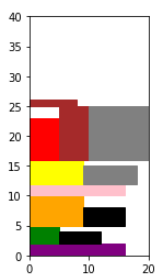
\includegraphics[width=0.5\linewidth]{6_con_rotar.jpg}}
%\caption{Grafico de Instancia SPPA13 con rotacion }
%\label{fig_12}
%\end{figure} 

Podemos observar como el permitir rotaciones de rectangulos se aprovecha mejor es espacio de la tira para todas las instancias, reduciendo asi la cantidad de desperdicio de forma sustancial. Para este tipo de problemas de alta complejidad vemos que los algoritmos geneticos tienen un desempeño mas que aceptable, siendo una excelente forma de encarar este tipo de problemas.


\section{Conclusiones}
Dada la simplesa de los algoritmos y su desempeño a la hora de encontrar una solucion eficiente, las metaheuristicos poblacionales, en este caso Algoritmos Geneticos, son una excelente forma de atacar problemas de complejidad NP hard cuya funcion de evaluacion sea simple (minimo valor posible) como es el caso de SPP, problema que surje en distintas areas ademas de las obvias como pueden ser aprovechamiento de material (madera, vidrio, metal,etc) como en la computacion donde se modelan jobs que requieren una parte contigua de la memoria durante un período de tiempo determinado entre otros.

Por ultimo, los GA, son una prometedora herramienta para la industria.

%------------------------------------------------ 
\section*{Agradecimientos}
Prof. Guillermo Leguizamon

%----------------------------------------------------------------------------------------
%	Listado de bibliografía consultada / Puede incluír sitios web
%----------------------------------------------------------------------------------------

\begin{thebibliography}{99} % Bibliography - this is intentionally simple in this template
\bibitem0.\t[Clinton Sheppard, 2018]{}Genetic Algorithms with Python
\bibitem1.\t[Wikipedia]{}\url{https://en.wikipedia.org/wiki/Genetic_algorithm}
\bibitem2.\t[Wikipedia]{}\url{https://en.wikipedia.org/wiki/Evolutionary_computation}
\bibitem3.\t[Wikipedia]{}\url{https://en.wikipedia.org/wiki/Gradient_descent}
\bibitem4.\t[Wikipedia]{}\url{https://en.wikipedia.org/wiki/Quasi-Newton_method}
\bibitem5.\t[Cornell University - Ithaca, New York]{}\url{https://arxiv.org/abs/1308.4008v1} A Literature Survey of Benchmark Functions For Global Optimization Problems




\end{thebibliography} 
 
\section{Código del Algoritmo}
\begin{lstlisting}[language=Python]

def genetiquear():
	while(not finish):
		print("codeando")
return "code"

\end{lstlisting}
\newpage
\tableofcontents
\end{document}